\documentclass[11pt]{article}

\usepackage[a4paper,margin=2.2cm]{geometry}
\usepackage{amsmath,amssymb}
\usepackage{graphicx}
\usepackage{subcaption}
\usepackage{booktabs}
\usepackage{siunitx}
\usepackage{xcolor}
\usepackage[hidelinks]{hyperref}
\usepackage{caption}
\captionsetup{font=small}

\newcommand{\ts}{t_{s}}
\newcommand{\tox}{t_{ox}}
\newcommand{\Wdep}{W}
\newcommand{\BV}{\mathrm{BV}}
\newcommand{\Ei}{\mathrm{Ei}}

\title{\vspace{-1.2cm}\textbf{Reproduction of Merchant, Arnold, Baumgart, Mukherjee,
Pein \& Pinker (ISPSD 1991)}\\[4pt]
\large ``Realization of High Breakdown Voltage ($>$700\,V) in Thin SOI Devices''\\
\normalsize Proc.\ ISPSD 1991, pp.~31--35}
\author{Independent derivation, simulation and figure-by-figure comparison,\\
with an extension to 4H-SiC and GaN films}
\date{}

\begin{document}
\maketitle
\vspace{-0.8cm}

\begin{abstract}
\noindent A lateral P$^+$--N SOI diode's breakdown voltage is maximized, for a
given lateral depletion width $\Wdep$, by choosing the doping profile $N(x)$
that makes the lateral field $E_x$ laterally uniform rather than the usual way
around (doping $\to$ field). The paper derives the resulting closed-form field
distribution, an avalanche-breakdown model via two dominant ionization paths,
and shows --- experimentally and theoretically --- that breakdown voltage
\emph{increases} as the SOI film thins below $\sim$\SI{1}{\micro\meter},
because the silicon's own critical field rises faster than the shrinking
ionization path length loses. This note reproduces the closed-form model
(Figs.~3--5), and extends it, unchanged, to 4H-SiC and GaN films using
literature Chynoweth ionization fits.
\end{abstract}

\section*{Key results (model vs.\ paper)}
\begin{center}
\begin{tabular}{@{}lcc@{}}
\toprule
Quantity & Model & Paper \\
\midrule
Oxide breakdown voltage, $\ts=\SI{0.1}{\micro\meter}$, $\tox=\SI{2}{\micro\meter}$ & \SI{1210}{\volt} & \SI{1200}{\volt} (Fig.~4 dashed line) \\
$\BV$, $\ts=\SI{0.1}{\micro\meter}$, $\tox=\SI{2}{\micro\meter}$, $\Wdep\to\infty$ & \SI{863}{\volt} & $\sim$\SI{865}{\volt} (Fig.~5 plateau) \\
$\BV$, $\ts=\SI{0.1}{\micro\meter}$, $\tox=\SI{2}{\micro\meter}$, $\Wdep=\SI{70}{\micro\meter}$ & \SI{849}{\volt} & \SI{750}{\volt} (Fig.~3, $L=\SI{70}{\micro\meter}$ device) \\
Design $\Wdep$ for $\BV=\SI{750}{\volt}$ (Fig.~3) & \SI{49.4}{\micro\meter} & $<L=\SI{70}{\micro\meter}$ \checkmark \\
\bottomrule
\end{tabular}
\end{center}

\section{Theory}

\subsection{The device and the design goal}
A lateral P$^+$--N diode sits in a thin SOI film over a buried oxide (BOX) on a
grounded N$^+$ substrate, shorted to the P$^+$ region (Fig.~2). $x$ is lateral
(0 at the P$^+$/N junction), $y$ vertical, downward. $\ts$, $\tox$ are the SOI
and buried-oxide thickness, $L$ the P$^+$-to-N$^+$ spacing, $\Wdep$ the lateral
depletion width at breakdown ($\Wdep<L$).

Unlike a conventional RESURF design, the paper works \emph{backward}: it picks
the field distribution that maximizes breakdown voltage for a given $\Wdep$
--- a laterally \emph{uniform} $E_x$, independent of $y$ --- then derives the
lateral doping $N(x)$ that produces it via Poisson's equation.

\subsection{Closed-form field and potential}
Gauss's law and the uniform-$E_x$ condition (paper eqs.~2--4) give, with
$E_y(x,0)=0$ (full depletion, minimum surface field) and
$\phi(x,0)=Vx/\Wdep$ (linear top-surface potential):
\begin{align}
E_y(x,y) &= \frac{Vxy}{t\,\Wdep\,\ts}, \\
E_x(y) &= -\frac{V}{\Wdep}\left(1-\frac{y^2}{2\ts t}\right), \\
t &= \frac{\ts}{2} + \frac{K_s}{K_{ox}}\tox, \qquad \frac{K_s}{K_{ox}}=\frac{11.7}{3.9}=3,
\end{align}
for $0\le x\le\Wdep$, $0\le y\le\ts$. $t$ is the effective series thickness of
half-depleted silicon plus $3\times$ the oxide (the Si/oxide
displacement-continuity jump). $E_x$ peaks at $y=0$; $E_y$ peaks at the corner
$(x=\Wdep,y=\ts)$. Integrating the resulting $Q(x)$ shows the required lateral
doping is \emph{linear} in $x$ --- the SOI analogue of the
Stengl--G\"osele ``variation of lateral doping'' concept the paper cites.
The potential itself (used to reproduce Fig.~3) is
\begin{equation}
\phi(x,y) = \frac{Vx}{\Wdep}\left(1-\frac{y^2}{2tt_s}\right), \qquad 0\le y\le \ts,
\end{equation}
continuing linearly in $y$ through the charge-free oxide beneath.

\subsection{Avalanche breakdown}
Ionization occurs only in the silicon, via the paper's own Chynoweth fit
(eq.~10):
\begin{equation}
\alpha(E) = a\,e^{-b/E}, \qquad a = \SI{7.03e5}{\per\centi\meter},\;\;
b = \SI{1.468e6}{\volt\per\centi\meter}
\end{equation}
(valid $\SI{1.75e5}{}\le E\le\SI{6.4e5}{\volt\per\centi\meter}$; a different $b$
than Nakagawa 1990's high-field branch). Two generation points dominate:

\textbf{Path 1} --- at $y=0$ where $|E_x|$ is largest (and, by design, constant
across $0<x<\Wdep$): identical to a 1-D p-i-n diode of width $\Wdep$,
\begin{equation}
I_1 = a\Wdep\,e^{-b\Wdep/V}. \label{eq:I1}
\end{equation}

\textbf{Path 2} --- at the corner $(x=\Wdep,y=\ts)$ where $|E_y|$ is largest: a
vertical leg through the silicon depth (closed form via the exponential
integral $\Ei$) plus a horizontal leg back along $y=\ts$,
\begin{align}
I_2' &= a\ts\gamma\Big[\Ei(-\gamma)+\frac{e^{-\gamma}}{\gamma}\Big],
\qquad \gamma=\frac{bt}{V}, \label{eq:I2p}\\
I_2'' &= a\Wdep\exp\!\left(-\frac{b\Wdep}{V(1-\ts/2t)}\right). \label{eq:I2pp}
\end{align}
Breakdown is the lowest $V$ solving $(1-I_1)(1-I_2'-I_2'')=0$, i.e.\ the
lowest $V$ at which $\max(I_1,I_2'+I_2'')$ first reaches~1.

\subsection{Why thinner SOI can raise the breakdown voltage}
As $\Wdep\to\infty$, $I_1$ and $I_2''$ vanish (they decay like
$\Wdep e^{-\mathrm{const}\cdot\Wdep}$), leaving only $I_2'(V,\ts,\tox)=1$ to
solve --- a $\BV(\ts,\tox)$ relation independent of $\Wdep$ (Fig.~4). A shorter
silicon path (smaller $\ts$) needs a \emph{higher} critical field to reach
ionization integral~1, exactly as in a one-sided step junction. Below
$\ts\sim\SI{1}{\micro\meter}$ this effect overtakes the ``shorter path''
effect, so $\BV$ rises again as $\ts$ falls --- the characteristic ``U'' shape
of Fig.~4 --- until the buried oxide's own dielectric strength
($\sim\SI{600}{\volt\per\micro\meter}$) caps the achievable $\BV$.

\section{Figure-by-figure comparison}

\begin{figure}[h!]
\centering
\begin{subfigure}{0.46\textwidth}
\includegraphics[width=\linewidth]{../figs_paper/fig3_paper_crop.png}
\caption{Paper (original)}
\end{subfigure}\hfill
\begin{subfigure}{0.52\textwidth}
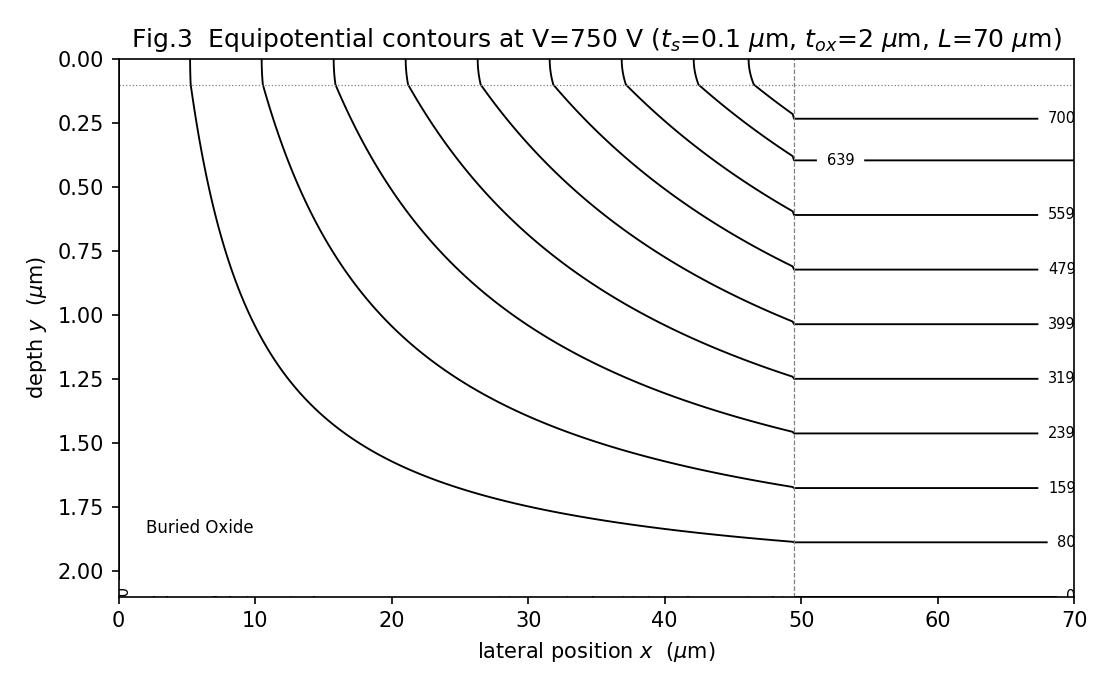
\includegraphics[width=\linewidth]{../figs/fig3_potential.png}
\caption{This reproduction}
\end{subfigure}
\caption{\textbf{Fig.~3 --- equipotential contours} ($\ts=\SI{0.1}{\micro\meter}$,
$\tox=\SI{2}{\micro\meter}$, $L=\SI{70}{\micro\meter}$), at the breakdown
voltage. The model plots the closed-form $\phi(x,y)$ directly --- no numerical
Poisson solve is needed, since the paper's whole design is a closed-form field.
The design width $\Wdep=\SI{49.4}{\micro\meter}$ is found by inverting
$\BV(\Wdep)=\SI{750}{\volt}$ to match the paper's stated result.}
\end{figure}

\begin{figure}[h!]
\centering
\begin{subfigure}{0.46\textwidth}
\includegraphics[width=\linewidth]{../figs_paper/fig4_paper_crop.png}
\caption{Paper (original)}
\end{subfigure}\hfill
\begin{subfigure}{0.52\textwidth}
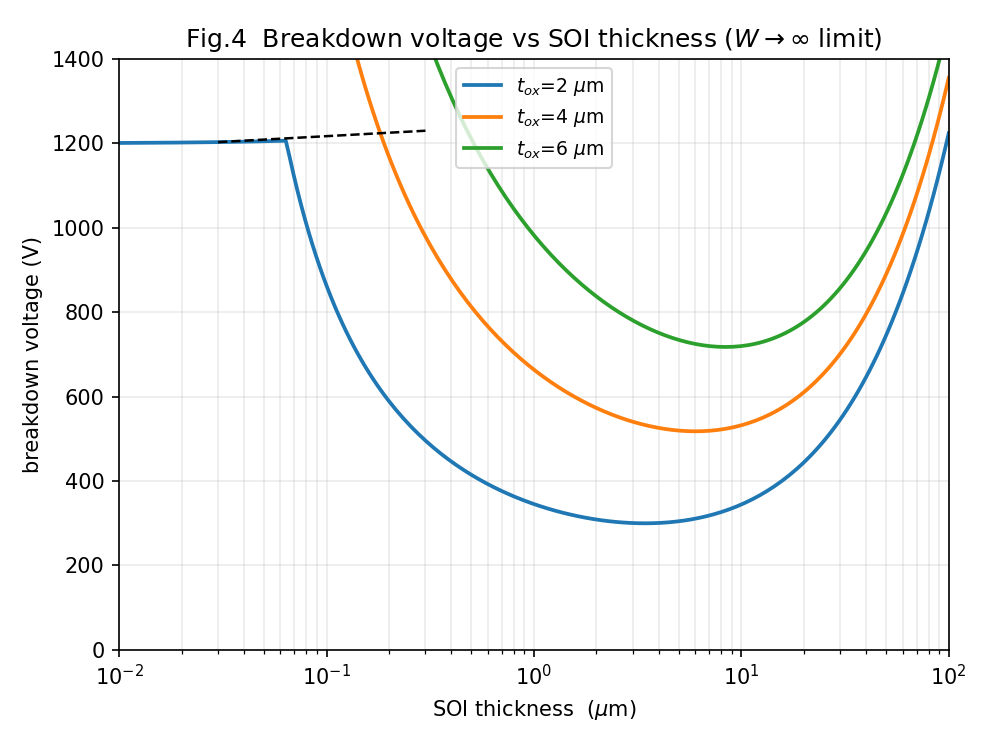
\includegraphics[width=\linewidth]{../figs/fig4_bv_vs_ts.png}
\caption{This reproduction}
\end{subfigure}
\caption{\textbf{Fig.~4 --- breakdown voltage vs.\ SOI thickness}
($\Wdep\to\infty$ limit), for $\tox=2/4/6\,\si{\micro\meter}$. The
characteristic ``U'' shape and the oxide-breakdown cap
(\SI{1210}{\volt} modeled vs.\ \SI{1200}{\volt} paper) reproduce closely.
The absolute $\BV$ level runs $\sim$15\% higher than the paper's text (``700\,V
may be achieved''); since Fig.~5's plateau and the oxide cap both match
closely, this is most likely the paper's rounded reference to its
$>$700\,V experimental headline rather than a precise Fig.~4 graph reading.}
\end{figure}

\begin{figure}[h!]
\centering
\begin{subfigure}{0.46\textwidth}
\includegraphics[width=\linewidth]{../figs_paper/fig5_paper_crop.png}
\caption{Paper (original)}
\end{subfigure}\hfill
\begin{subfigure}{0.52\textwidth}
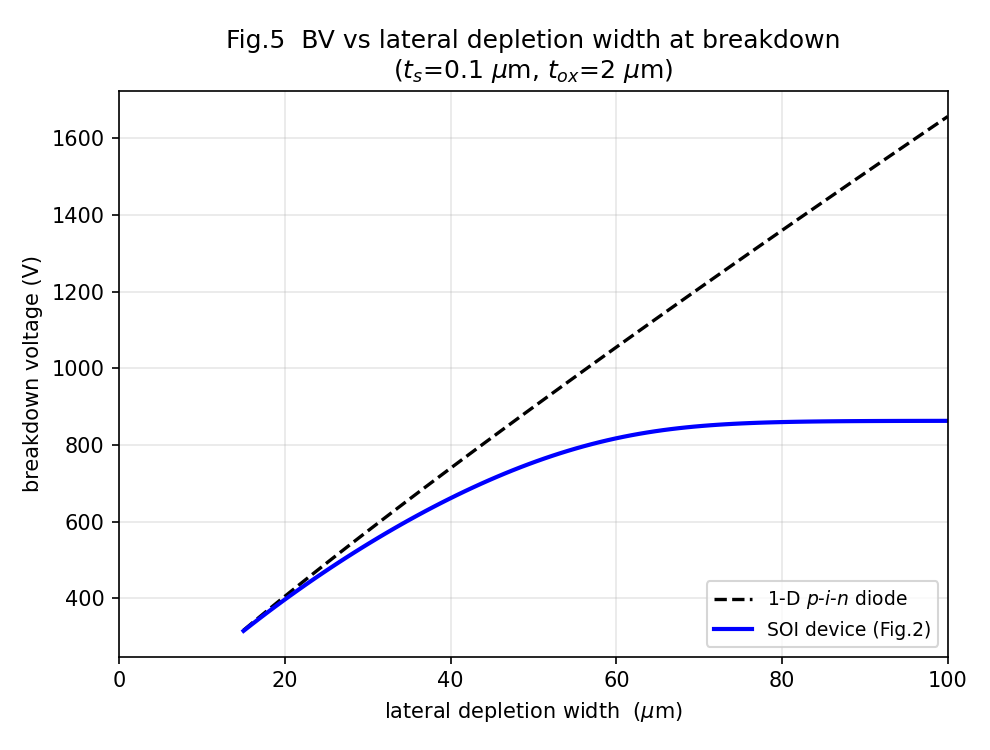
\includegraphics[width=\linewidth]{../figs/fig5_bv_vs_W.png}
\caption{This reproduction}
\end{subfigure}
\caption{\textbf{Fig.~5 --- breakdown voltage vs.\ lateral depletion width}
$\Wdep$ ($\ts=\SI{0.1}{\micro\meter}$, $\tox=\SI{2}{\micro\meter}$), vs.\ the
1-D p-i-n reference. Excellent match: both the SOI-device saturation
($\sim$863--870\,V) and the linear p-i-n reference track the paper closely
over the full range.}
\end{figure}

\clearpage
\section{Extension --- 4H-SiC and GaN films}

Nothing in Sec.~1 is silicon-specific except the single-carrier Chynoweth
ionization fit and the film's relative permittivity $K_s$ (the buried oxide
stays SiO$_2$, $K_{ox}=3.9$). Swapping in literature Chynoweth fits for 4H-SiC
and GaN re-evaluates the \emph{same} closed-form model
(\texttt{model.py}'s \texttt{Material}/\texttt{MATERIALS} registry) for a
wide-bandgap-on-insulator version of the device.

\begin{center}
\begin{tabular}{@{}lccl@{}}
\toprule
Material & $K_s$ & $a$ (\si{\per\centi\meter}), $b$ (\si{\volt\per\centi\meter}) & Source \\
\midrule
Si & 11.7 & $7.03\times10^5$, $1.468\times10^6$ & Merchant et al.\ 1991, eq.~10 \\
4H-SiC & 9.7 & $3.25\times10^6$, $1.71\times10^7$ & Raghunathan \& Baliga, APL \textbf{72}, 3503 (1998), holes \\
GaN & 8.9 & $6.4\times10^5$, $1.454\times10^7$ & Cao et al., APL \textbf{112}, 262103 (2018), holes \\
\bottomrule
\end{tabular}
\end{center}

\subsection{Result: the oxide, not the film, limits at this design point}
At the paper's own design point ($\ts=\SI{0.1}{\micro\meter}$,
$\tox=\SI{2}{\micro\meter}$, $\Wdep\to\infty$), 4H-SiC's and GaN's much larger
$b$ (higher ionization threshold field) implies enormous semiconductor-limited
breakdown voltages if the film alone is considered:

\begin{center}
\begin{tabular}{@{}lcccc@{}}
\toprule
Material & Semiconductor-limit BV & Oxide cap & Actual (capped) BV & Oxide/film crossover $\ts$ \\
\midrule
Si & \SI{863}{\volt} & \SI{1210}{\volt} & \SI{863}{\volt} & \SI{0.064}{\micro\meter} \\
4H-SiC & \SI{3990}{\volt} & \SI{1212}{\volt} & \SI{1212}{\volt} & \SI{32.8}{\micro\meter} \\
GaN & \SI{6947}{\volt} & \SI{1213}{\volt} & \SI{1213}{\volt} & \SI{28.8}{\micro\meter} \\
\bottomrule
\end{tabular}
\end{center}

But the buried SiO$_2$ breaks down first for both wide-bandgap materials:
its dielectric strength ($\SI{600}{\volt\per\micro\meter}$, unchanged) caps
all three materials at essentially the same $\sim$\SI{1210}{}--\SI{1213}{\volt},
since the oxide cap is set almost entirely by $\tox$ once $\ts\ll\tox$.
\textbf{In this architecture, at this film thickness, 4H-SiC and GaN gain
nothing over silicon.}

\subsection{A closed-form, $\tox$-independent crossover}
Both $\BV$ (the $\Wdep\to\infty$ semiconductor limit) and the oxide breakdown
voltage $V_{ox}$ are proportional to the same $t=\ts/2+(K_s/K_{ox})\tox$:
$\BV = bt/\gamma^\ast(\ts)$, where $\gamma^\ast(\ts)$ is the root of
eq.~\eqref{eq:I2p}'s $I_2'=1$ condition, and
$V_{ox}=E_{ox,\mathrm{crit}}\,t/(K_s/K_{ox})$. Setting $\BV=V_{ox}$, the
common factor $t$ \emph{cancels}, leaving a condition on $\ts$ alone:
\begin{equation}
\gamma_{\mathrm{cross}} = \frac{b\,(K_s/K_{ox})}{E_{ox,\mathrm{crit}}},
\qquad
a\,\ts\,\gamma_{\mathrm{cross}}\Big[\Ei(-\gamma_{\mathrm{cross}})
+\frac{e^{-\gamma_{\mathrm{cross}}}}{\gamma_{\mathrm{cross}}}\Big] = 1.
\end{equation}
\textbf{The oxide/film crossover thickness is exactly independent of
$\tox$} --- a closed-form fact of the model
(\texttt{model.crossover\_film\_thickness}), not a numerical coincidence,
confirmed by brute-force root-finding across $\tox$ in Fig.~\ref{fig:crossover}.
Silicon's crossover (\SI{0.064}{\micro\meter}) sits right at the edge of the
paper's own thin-film regime, which is why Si's Fig.~4 ``U'' is genuinely
film-limited over most of its interesting range. 4H-SiC's and GaN's crossover
thicknesses ($\sim$29--33\,\si{\micro\meter}) are two orders of magnitude
larger: \textbf{the whole point of this paper --- pushing the film to
sub-micron thickness to raise BV --- does not transfer to wide-bandgap films
with a plain \SI{2}{\micro\meter} SiO$_2$ BOX}, because at any sub-micron
thickness they are deep in the oxide-limited regime. Exploiting 4H-SiC's or
GaN's intrinsic advantage in this architecture would require either a much
thicker buried oxide or a higher-dielectric-strength insulator, not a thinner
film.

\begin{figure}[h!]
\centering
\begin{subfigure}{0.32\textwidth}
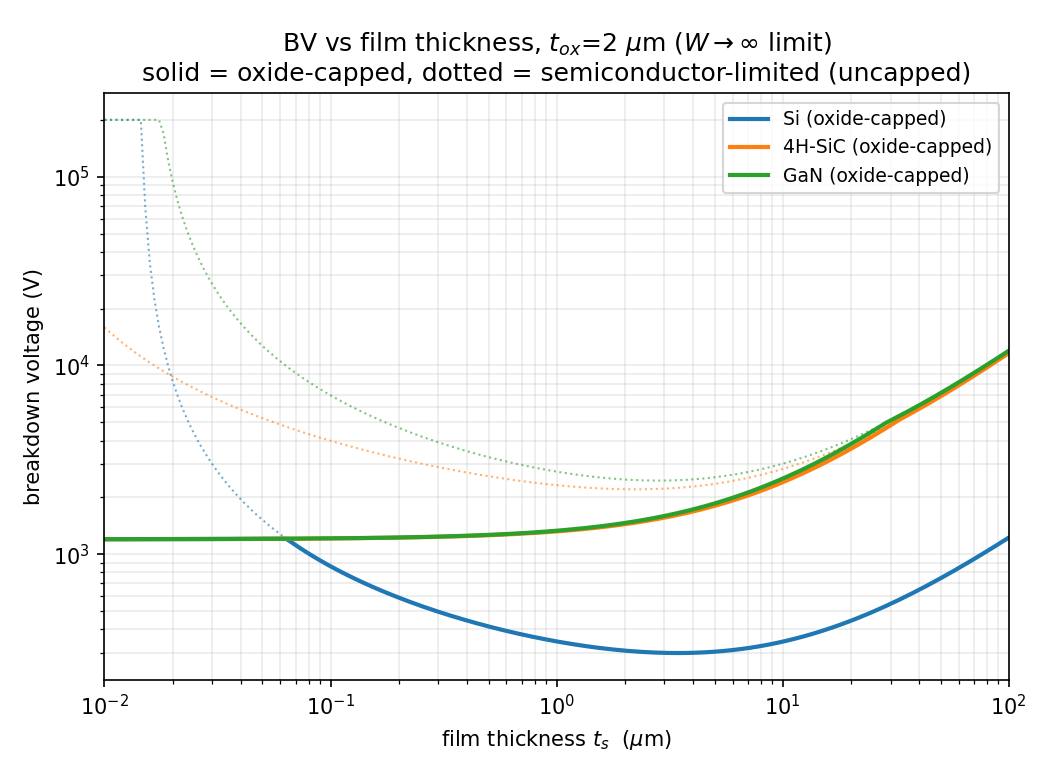
\includegraphics[width=\linewidth]{../figs/fig4_materials.png}
\caption{BV vs.\ film thickness, $\tox=\SI{2}{\micro\meter}$}
\end{subfigure}\hfill
\begin{subfigure}{0.32\textwidth}
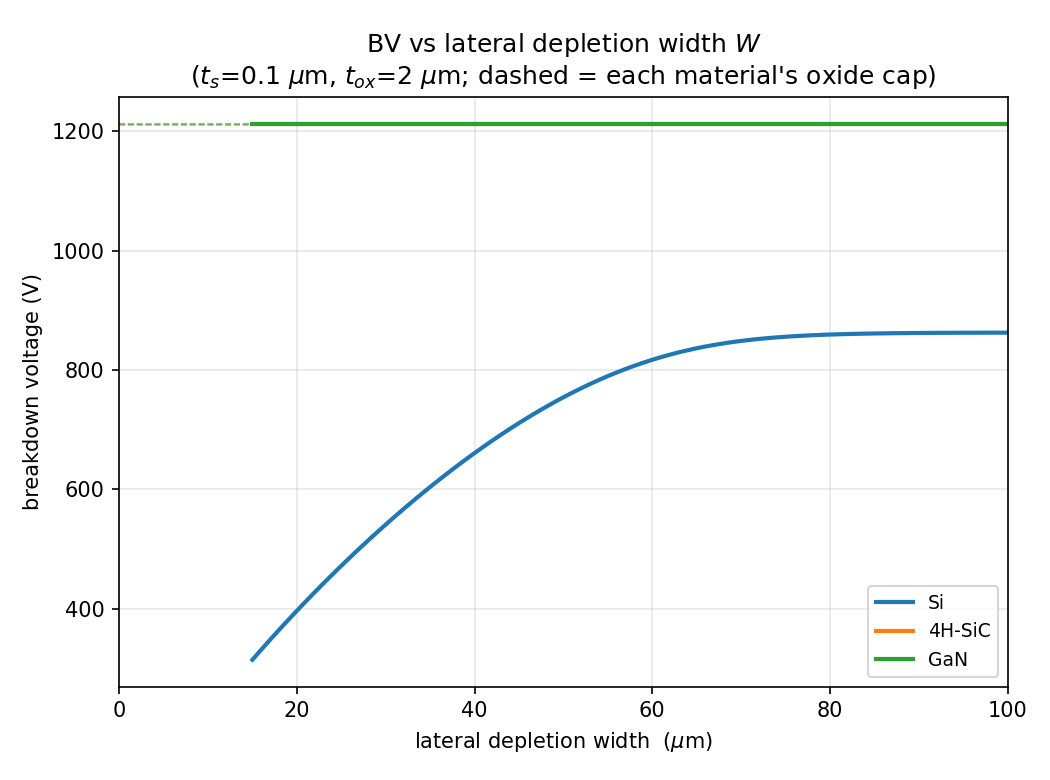
\includegraphics[width=\linewidth]{../figs/fig5_materials.png}
\caption{BV vs.\ lateral depletion width $\Wdep$}
\end{subfigure}\hfill
\begin{subfigure}{0.32\textwidth}
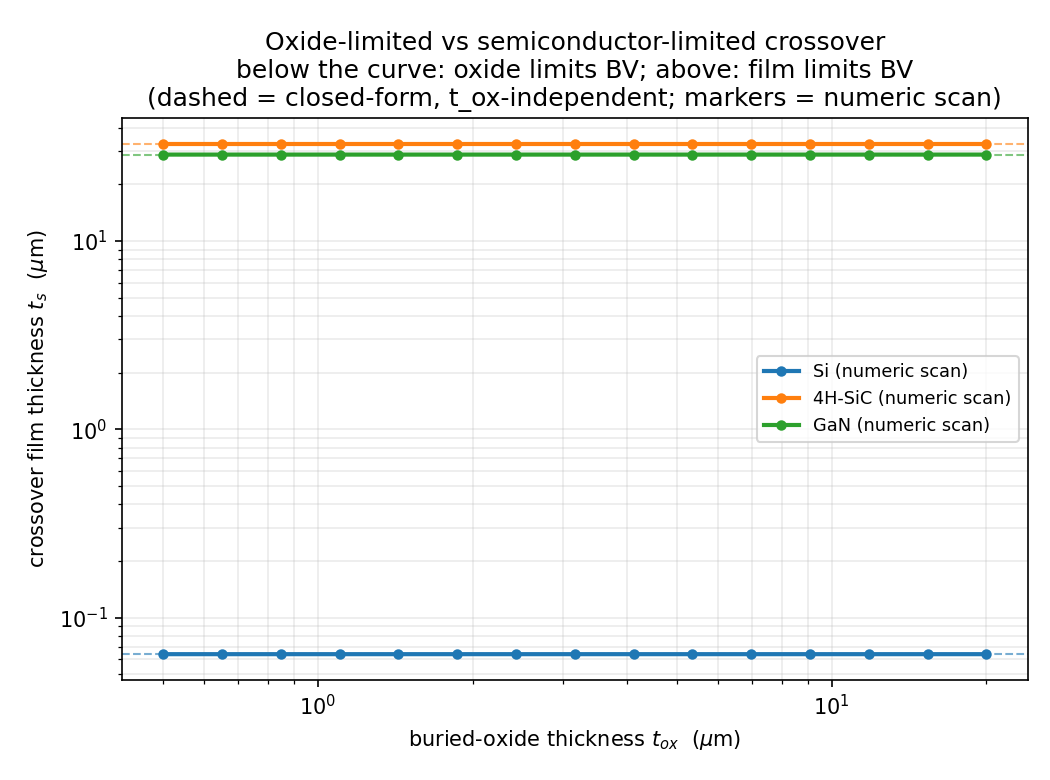
\includegraphics[width=\linewidth]{../figs/fig_oxide_crossover.png}
\caption{Oxide/film crossover $\ts$}
\end{subfigure}
\caption{\textbf{4H-SiC / GaN extension} (model-only; no corresponding paper
figure). (a) Solid = oxide-capped (actual), dotted = semiconductor-limited
(uncapped). (b) $\ts=\SI{0.1}{\micro\meter}$, $\tox=\SI{2}{\micro\meter}$;
dashed = each material's oxide cap. (c) Crossover film thickness $\ts$ is
exactly independent of $\tox$ for all three materials (closed form matches
brute-force numerical scan).}
\label{fig:crossover}
\end{figure}

\clearpage
\section{The plateau problem --- why Si's BV($t_s$) minimum is broad}

Fig.~4's ``U'' curve has a minimum in $\ts$; visually, silicon's is a broad,
flat plateau while 4H-SiC's and GaN's are narrow, sharp ``V''s. This follows
from an exact factorization of the model already used above:
\begin{equation}
V_{BR}(\ts,\tox) = E_c(\ts)\cdot t_{eff}(\ts,\tox), \qquad
E_c(\ts) := \frac{b}{\gamma^\ast(\ts)},
\end{equation}
where $\gamma^\ast(\ts)$ is the root of $a\,\ts\,\gamma\big[\Ei(-\gamma)+e^{-\gamma}/\gamma\big]=1$
--- an equation in $\ts$ and the material's ionization prefactor $a$
\emph{alone} (\texttt{model.g\_star}, \texttt{model.critical\_field}); neither
$\tox$ nor $K_s$ enters $E_c(\ts)$ at all (verified numerically to solver
tolerance). Taking logarithmic derivatives, $dV_{BR}/d\ts=0$ where
\begin{equation}
\underbrace{-\frac{d\ln E_c}{d\ln \ts}}_{\text{material \& }\ts\text{ only}}
\;=\;
\underbrace{\frac{\ts/2}{\ts/2 + r\,\tox}}_{\text{material's }r\text{, }\ts\text{, }\tox},
\qquad r = \frac{K_s}{K_{ox}}. \label{eq:plateau}
\end{equation}
This crossing was checked against a direct numerical minimization of
$V_{BR}(\ts)$ for all 9 (material, $\tox$) combinations tested: it locates the
minimum to within \SI{0.01}{\micro\meter} every time.

\textbf{Why Si's plateau is broader.} The LHS of \eqref{eq:plateau} depends on
material only through $a$ (not $b$, not $K_s$). Si's Chynoweth $b$ is
$\sim$10$\times$ smaller than 4H-SiC's/GaN's, so its critical field's
log-slope varies far more gently with $\ts$; a gently-varying LHS stays
nearly matched to the slowly-varying, bounded RHS over a \emph{wide} $\ts$
range (broad plateau), while a steeply-varying LHS (4H-SiC, GaN) crosses
sharply at one point (narrow ``V'').

\textbf{Quantified.} Defining the plateau width as the $\ts$-interval around
the numerically-found minimum over which $|dV_{BR}/d\ts|/V_{BR,\min}$ stays
below 1\%/\si{\micro\meter}:
\begin{center}
\begin{tabular}{@{}lccc@{}}
\toprule
$\tox$ & Si & 4H-SiC & GaN \\
\midrule
\SI{2}{\micro\meter} & \SI{1.19}{\micro\meter} & \SI{0.58}{\micro\meter} & \SI{0.73}{\micro\meter} \\
\SI{4}{\micro\meter} & \SI{4.47}{\micro\meter} & \SI{2.27}{\micro\meter} & \SI{2.78}{\micro\meter} \\
\SI{6}{\micro\meter} & \SI{13.03}{\micro\meter} & \SI{5.24}{\micro\meter} & \SI{6.34}{\micro\meter} \\
\bottomrule
\end{tabular}
\end{center}
Si's plateau is consistently $\sim$2$\times$ wider than 4H-SiC's or GaN's at
the same $\tox$; permittivity (entering only through the RHS) is a secondary
effect, the dominant cause being Si's much weaker field-sensitivity of impact
ionization ($b$), not permittivity.

\begin{figure}[h!]
\centering
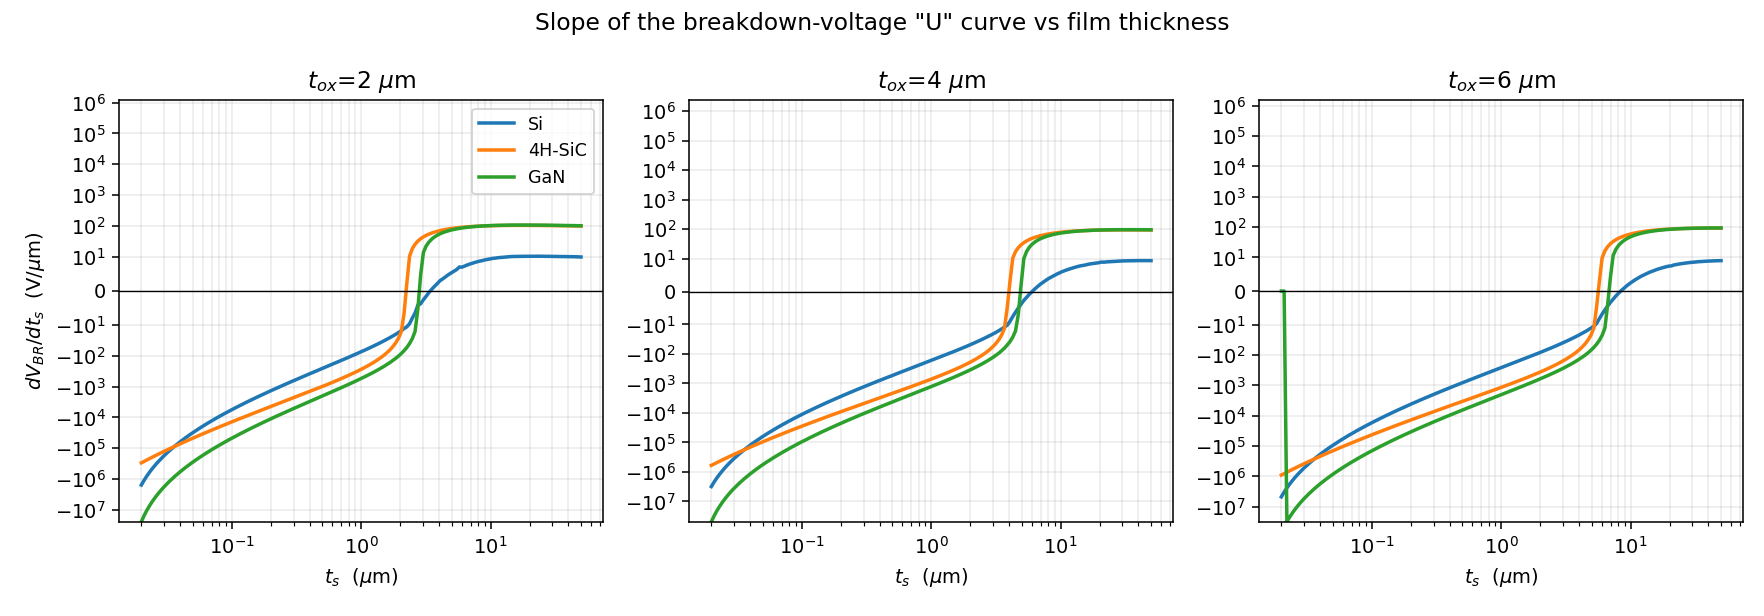
\includegraphics[width=0.92\linewidth]{../figs/fig_dbv_dts.png}
\caption{\textbf{Raw derivative $dV_{BR}/d\ts$ vs.\ $\ts$}, Si/4H-SiC/GaN, one
panel per $\tox\in\{2,4,6\}\,\si{\micro\meter}$. The wider the flat region
around the zero-crossing, the broader the plateau.}
\end{figure}

\begin{figure}[h!]
\centering
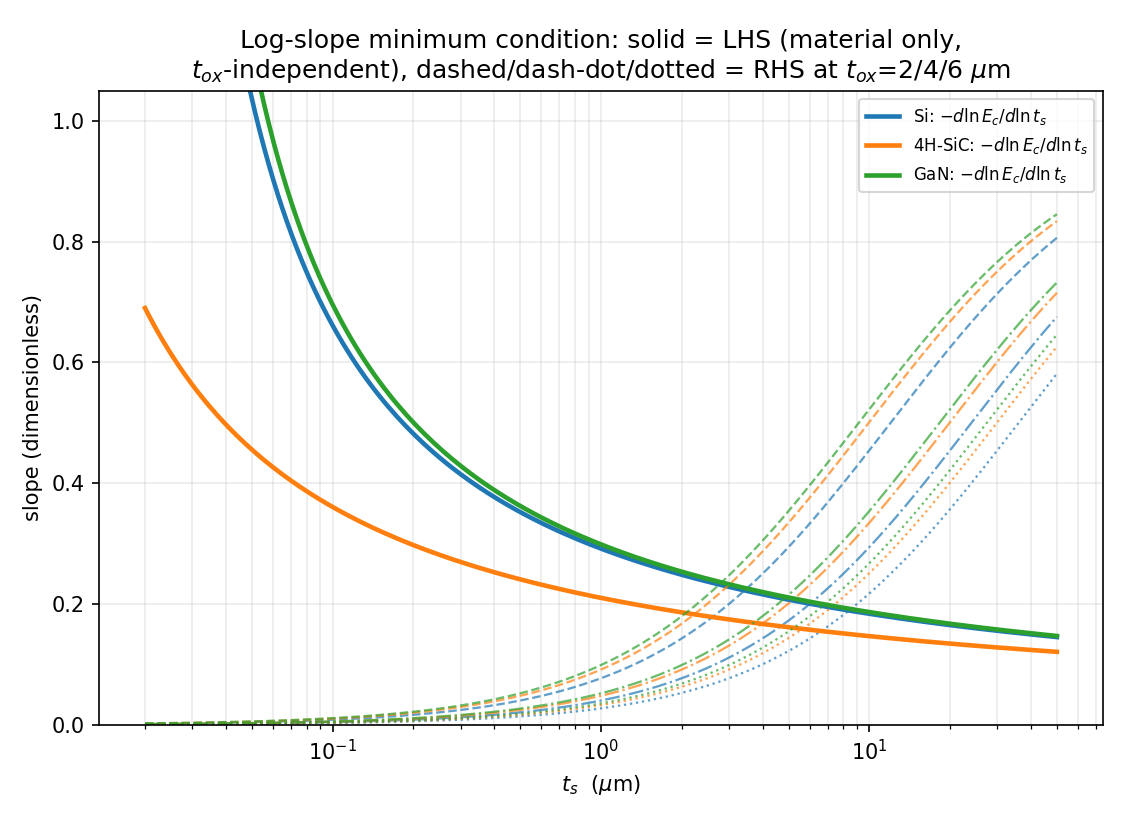
\includegraphics[width=0.7\linewidth]{../figs/fig_log_slope.png}
\caption{\textbf{Log-slope minimum condition} \eqref{eq:plateau}: solid = LHS
(material-only, $\tox$-independent); dashed/dash-dot/dotted = RHS at
$\tox=2/4/6\,\si{\micro\meter}$. Crossings match $V_{BR}(\ts)$'s numerical
minima to within \SI{0.01}{\micro\meter}.}
\end{figure}

\begin{figure}[h!]
\centering
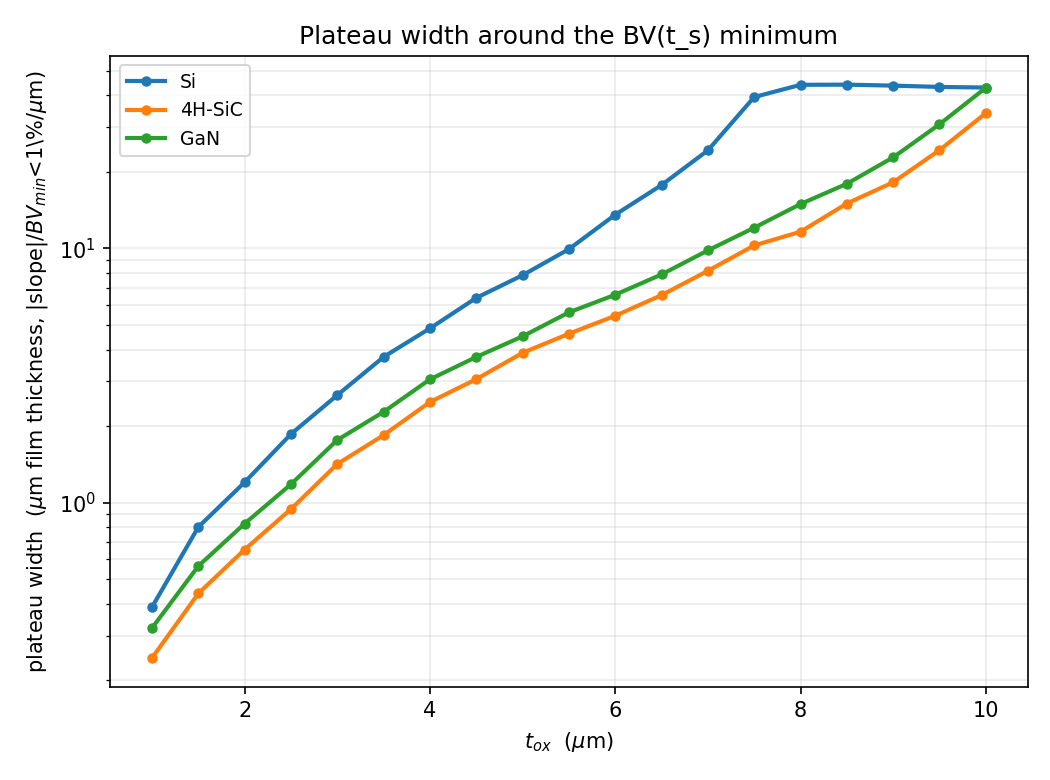
\includegraphics[width=0.7\linewidth]{../figs/fig_plateau_width.png}
\caption{\textbf{Plateau width vs.\ $\tox$}, per material --- Si is
consistently $\sim$2$\times$ wider than 4H-SiC or GaN at the same $\tox$.}
\end{figure}

\clearpage
\section{Notes and limitations}
\textbf{Fig.~6 (experimental I-V trace) --- out of scope.} Fig.~6 is a
photographed oscilloscope trace of a fabricated device; it is experimental
data, not a simulation target (\texttt{figs\_paper/fig6\_paper\_crop.png}
holds the original).\\[4pt]
\textbf{Known quantitative gap.} The absolute breakdown-voltage level in
Fig.~4 runs $\sim$15\% higher than the paper's text; however Fig.~5's
$\Wdep\to\SI{100}{\micro\meter}$ plateau ($\sim$\SI{865}{\volt}) and the
oxide-breakdown cap (\SI{1210}{} vs.\ \SI{1200}{\volt}) both match closely, so
the paper's ``700\,V'' text is most likely a rounded reference to the
$>$700\,V experimental headline rather than a precise Fig.~4 graph
reading.\\[4pt]
\textbf{Assumptions.} Ionization coefficients are the paper's own stated fit
(eq.~10), not the Van Overstraeten--de Man values used in later papers. Only
the two paper-identified dominant ionization paths are evaluated (eq.~13's
product formally has infinitely many paths). Fig.~3's device is assumed to
follow the derived linear $N(x)$ out to a single design width $\Wdep$; beyond
$\Wdep$ the SOI is treated as quasi-neutral at the applied bias. The 4H-SiC and
GaN fits use hole ionization coefficients for comparability across
materials --- see \texttt{model.py}'s docstring for the full reasoning.\\[4pt]
\textbf{Code:} \texttt{model.py} --- core closed-form fields, ionization
integrals, and the \texttt{Material} registry; \texttt{fig3\_potential.py},
\texttt{fig4\_bv\_vs\_ts.py}, \texttt{fig5\_bv\_vs\_W.py} --- one script per
reproduced paper figure; \texttt{fig\_materials\_comparison.py} --- the
4H-SiC/GaN extension and crossover analysis; \texttt{fig\_plateau\_analysis.py}
--- the $dV_{BR}/d\ts$, log-slope, and plateau-width figures of Sec.~4.

\end{document}
